\chapter{Практический раздел}

Функция распределения случайной величины, распределенной по равномерному закону:

\begin{figure}[H]
    \begin{center}
    \includegraphics[width=0.7\linewidth]{inc/all_dist_uni.pdf}
    \caption{$F_X(x), X \sim R(a, b)$}
    \label{fig:}
    \end{center}
\end{figure}

\newpage

Функция плотности распределения случайной величины, распределенной по равномерному закону:

\begin{figure}[H]
    \begin{center}
    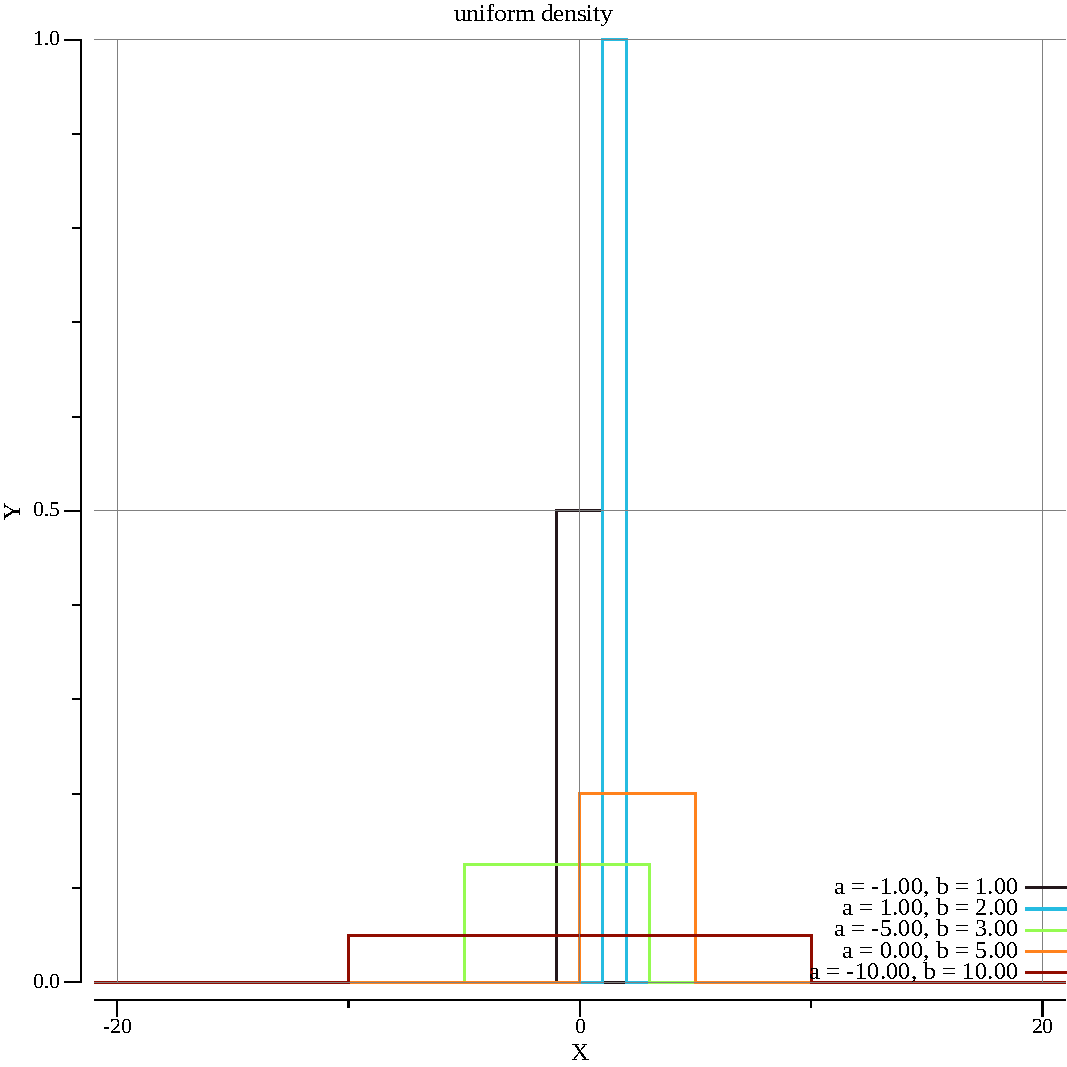
\includegraphics[width=0.7\linewidth]{inc/all_dens_uni.pdf}
    \caption{$f_X(x), X \sim R(a, b)$}
    \label{fig:}
    \end{center}
\end{figure}

Таким образом, при увеличении разности между $a$ и $b$ графики растягиваются по оси абсцисс, а график функции плотности распределения стягивается к 0 по оси ординат.

\newpage

Функция распределения случайной величины, распределенной по закону Эрланга:

\begin{figure}[H]
    \begin{center}
    \includegraphics[width=0.7\linewidth]{inc/all_dist_erl.pdf}
    \caption{$F_X(x), X \sim \Gamma(k, \lambda), k \in \mathbb {Z}$}
    \label{fig:}
    \end{center}
\end{figure}

При увеличении $k$ график растягивается по оси абсцисс. При увеличении $\lambda$ график стягивается по оси абсцисс.

\newpage

Функция плотности распределения случайной величины, распределенной по закону Эрланга:

\begin{figure}[H]
    \begin{center}
    \includegraphics[width=0.7\linewidth]{inc/all_dens_erl.pdf}
    \caption{$f_X(x), X \sim \Gamma(k, \lambda), k \in \mathbb {Z}$}
    \label{fig:}
    \end{center}
\end{figure}

При увеличении $k$ график растягивается по оси абсцисс, стягивается по оси ординат. При увеличении $\lambda$ график стягивается по оси абсцисс, растягивается по оси ординат.

\newpage

